\documentclass[a4paper,12pt]{article}
\usepackage[a4paper,margin=1in,footskip=0.25in]{geometry}
\usepackage[utf8]{inputenc}

% science
\usepackage{amsmath}
\usepackage{array}
\usepackage{siunitx}

% layout
\usepackage{float}
\usepackage{parskip}
\usepackage{graphicx}
\usepackage{circuitikz}
\usepackage{longtable}
\usepackage{hyperref}
\usepackage{subfig}

% referencing
\usepackage[style=apa]{biblatex}
\addbibresource{light.bib}
\usepackage{hyperref}

% table centering
\renewcommand{\arraystretch}{1.3}
\newcolumntype{P}[1]{>{\raggedright\arraybackslash}p{#1}}
\newcommand{\tptt}{$\times\,$}

% figures labelings
\usepackage{chngcntr}
\counterwithin{figure}{section}

% uncertainty
\newcommand{\absun}{\Delta \text{unc}\,}
\newcommand{\relun}{\% \text{unc}\,}

\newcommand{\paragraphnl}[1]{\textbf{#1}\\\\}


\title{Empirically finding the typical luminous efficacy of an incandescent light bulb through the inverse square law}
\author{Terry Qi}

\begin{document}

\maketitle

\section{Design}

\subsection{Introduction}
% personal
During the examination of a potential IA idea on the intensity of a refracted light-beam, I struggled with modeling a realistic light due to a lack of understanding and care towards the decrease in intensity of the light with respect to the distance. Because the glass cube I was working with had significant length, the decrease in intensity of the light-beam within the glass damaged my data and exponentially increased the difficulty in linearization. Therefore, I wanted to empirically see how the difference in distances will affect the measurement of light intensity. Additionally, I found the labs bulbs are prone to extreme heat even with little power and on duration. Thus, I thought to use this experiment to find the luminous efficacy of an incandescent lab light-bulb to confirm my suspicion.

\subsection{Research Question}
\begin{quote}
 What is the relationship between the distance to the light source in respect to the perceived illuminance?
\end{quote}

\subsection{Background}

For a light-bulb to produce light, an electrical current in the form of moving electrical charges must be presented and pass through a light emitting electrical resistor. While there exists difference in the efficiency of such resistors --- modern light emitting diodes (LED) are much more energetically efficient comparing to an incandescent light-bulb, the physical result: needed to illuminate a room through the emission of light waves in the visible spectrum, does not differ. Therefore, the theoretical definition of the rate of work, $P$, is only depended upon the level of electrical current (the flow rate of charges), and voltage (the work potential of charges), shown in figure \ref{eq:work}.

\begin{figure}[h!]
    \[
    P = IV
    \]
    \caption{The electrical definition of work}
    \label{eq:work}
\end{figure}

For it is the emission of light waves/photons that we call ``light'', the density of these photons in an area naturally defines the intensity of light (of units $\si{W\per m^2}$). This relationship is a part of the IB curriculum at topic 4.3, Waves Characteristics, where it states a fundamental property of light intensity --- that the intensity of light is proportional to the inverse distance squared (figure \ref{eq:prop}).

\begin{figure}[h!]
    \[
    I \propto \frac{1}{s^2}
    \]
    \caption{The inverse square relation}
    \label{eq:prop}
\end{figure}

Furthermore, if we consider the emission of these photons to be a perfect sphere around the light source, the density of photons at a given distance is simply represented via the surface area of the sphere with a radius of the distance.
%images
Using the unit definition of intensity, we can derive using the equation of the surface area of a sphere, the full intensity equation in figure \ref{eq:isl}:

\begin{figure}[h!]
    \[
    I = \frac{P}{\text{Area}} = \frac{P}{4\pi s^2}
    \]
    \caption{The inverse square law}
    \label{eq:isl}
\end{figure}

However, the human eyes does not perceive the intensity of light uniformly through the wavelengths \parencite{candela}. Under conditions for photopic vision --- the vision of the eye in a well lit area, we perceive light in the green wavelength (555 $\si{nm}$) the most intensely. Therefore there is a need for a unit that displays the normalized intensity of different wavelengths of light --- the unit Candela and the photopic luminosity function \parencite{si_candela}.

% talk about the relationship between
The intensity derived from the inverse square law (figure \ref{eq:isl}) is more formally known as the \textit{radiant intensity} \parencite{candela}, represented as a function of wavelength: $I_v(\lambda)$. By taking the incomplete integral on the weighted radiant intensity split into frequencies for all frequencies, we come to the definition of the \textit{luminous intensity} $I_v$, shown in figure \ref{eq:li}.

\begin{figure}[h!]
    \[
     I_v = K_{cd} \int_{0}^{\infty} V(\lambda) I_e(\lambda) \, d\lambda
    \]
    \caption{The definition of Luminous Intensity}
    \label{eq:li}
\end{figure}

Combining the notion of luminous intensity with the 3D generalized angle quantity, steradian ($\si{\ohm}$), we can derive the total luminous power ($\Phi_v$) created by the source, measured in unit lumen ($\si{lm}$),

\[
    \Phi_v = \si{\ohm} I_v,
\]

of which we can use to define the amount of luminous power incident on a surface through the quantity of illuminance, measured in units lux ($\si{lm\per m^2}$). The finalized relation is summarized in figure \ref{eq:dti}, \parencite{intensityLuminous_se}:

\begin{figure}[h!]
 \centering
 \begin{align*}
 I_e(\lambda) &= c(\lambda) \frac{P}{4\pi s^2}\\
  E_v &= \frac{1}{4\pi s^2 A} \si{\ohm} P K_{cd} \int_{0}^{\infty} V(\lambda) c(\lambda) \, d\lambda\\
  E_v & \propto P\frac{1}{s^2}
 \end{align*}
 \caption{The complete distance to illuminance relationship}
 \label{eq:dti}
\end{figure}

For the light sensor I have only measures intensity in lux, the above dive into luminosity serves as a justification for why I think the inverse square root applies to not just radiant intensity, but also to luminous intensity. Because the process of conversion is linear, it seems reasonable to hypothesize that illuminance is proportional to the distance squared.

To test my hypothesis, I thought to conduct the experiment on the small 5W lab light-bulbs, for they have a tendency to heat up quickly before. Through some preliminary testing, I decided to decrease the supply voltage: the bulb gets dangerously hot on 12V, and placing sensor no closer than 3cm, and no further than 10cm, for at too close the illuminance exceeds the limits of the sensor, and that illuminance quickly drops off from the starting value, bringing no need of longer distances.

Additionally, I figured to connect a voltmeter along side the ammeter. This is to measure the power of the light source, but the voltmeter is significant in that I do not trust the supply voltage of the power supply. I may be able to use the power measurement to calculate the luminous efficacy later on.

\subsection{Variables}
\paragraph{Independent Variable}
The distance the light sensor is to the light source measured in centimeters.

\paragraph{Dependent Variable}
The illuminance of the area measured by the light sensor at the distance in unit lux.

\subsection{Control Variables}

\begin{longtable}{P{0.2\textwidth}|P{0.35\textwidth}|P{0.35\textwidth}}
Controls & Reason & How\\\hline
Environmental room intensity & Systematically increase the the measured illuminance of the light-ray from the light-box & Conduct the experiment in a dark room, and record the ambient illuminance of the room \\
The sensitivity of the light sensor & Light sensors are sensitive to angular tilts, and a disturbed sensor due to shaky hands most likely will produce random errors throughout the experiment & Use strong tape to clamp down the light sensor at the given distance\\
Fluctuation of the outside light level & Environment lighting will leak through the lab windows, and have the ability to systematically change the measurements for a small time period & Conduct the experiment early in the morning or late at night, as to minimize the impacts from the sun\\
The power supplied to the light-bulb & Higher power will increase intensity at all distances, as shown in figure \ref{eq:isl}, causing systematic errors & Assert the connected ammeter and voltmeter readings are unchanged after changing the independent variable, the distance\\
The temperature of the bulb filament & For the resistance of a resistor tend to increase as it is heated, electrical current may fall in value, decreasing the power supplied, creating systematic errors & It is discouraged to directly touch the light-bulbs. Thus it is best to conduct the experiment quickly in time, as to minimize the possible heating up of the light-bulb.

\end{longtable}

\subsection{Materials}
\begin{itemize}
 \item Vernier light sensor ($\pm 2\si{lx}$) \parencite{vernier_manual} \& connection hub
 \item laptop with Vernier Data Logger software
 \item 5W light-bulb
 \item 5 wires
 \item 12V power supply
 \item digital ammeter ($\pm 0.1\si{A}$) and voltmeter ($\pm 0.1\si{V}$)
 \item one meter long ruler ($\pm 0.1\si{cm}$)
 \item reasonable supply of duct tape
 \end{itemize}

\subsection{Method}

\begin{enumerate}
 \item Choose a location with the least amount of ambient light, ideally early morning or at night.

 \item Connect the Vernier light sensor to the laptop, set light sensor's range to (0–6000 \si{lx}). Enable ``Statistics'' in the Vernier logger lite software by clicking ``Stats''.

 \item Set up the electrical circuit as shown in diagram \ref{fig:cd}, set the power supply voltage to 8V, with a digital ammeter and voltmeter. Allow the light-bulb to be in contact with the ground.

 \item Align the meter wooden ruler perpendicularly to the light-bulb, position the Vernier light sensor parallel to the ruler at a distance of 3cm to the light-bulb. The final layout should be similar to figure \ref{fig:layout}.

 \item Secure down the light sensor at distances of 3cm to 10cm, step 1cm, of a total of 8 distances.

 \item For each distance, record the readings on the ammeter and voltmeter, retry the measurement if they differ from the last distance. Record the illuminance over 10 seconds in the software, and note down the average illuminance value. Repeat the illuminance recording 5 times at the same distance.
\end{enumerate}

\subsection{Diagrams}

% circuit
\begin{figure}[h!]
\centering
\begin{circuitikz} \draw
    (0,3) to[battery,a=8V] (5,3) -- (5,0)
    to[lamp,a=5W] (0,0)
    to[ammeter] (0,3)
    (1,0) -- (1,-1.5)
    to[voltmeter] (4,-1.5) -- (4,0)
    ;
\end{circuitikz}
\caption{The circuit diagram of the setup}
\label{fig:cd}
\end{figure}

% diagram
% annotated picture, & a software screen
\begin{figure}[h!]
 \centering
 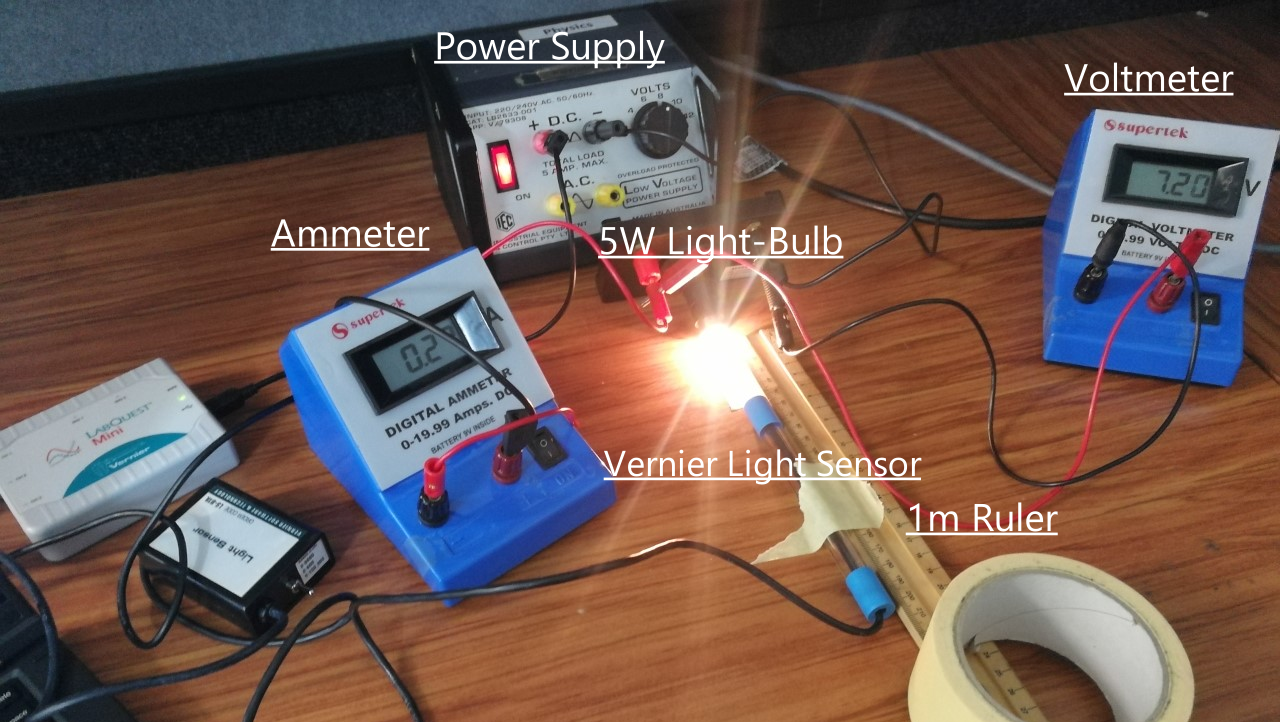
\includegraphics[width=\textwidth]{assets/setuppic.png}
 \caption{The experiment layout}
 \label{fig:layout}
\end{figure}


\subsection{Safety}
Avoid direct contact with exposed parts of the wires, additionally ensure a dry hand during the experiment. This will reduce the chance of an electrical accident.

Avoid touching the light-bulb throughout the experiment. The light-bulb got super hot during my experiment and direct skin contract may incur burns.

\section{Data}
\subsection{Raw data}
\begin{figure}[h!]
    \centering
    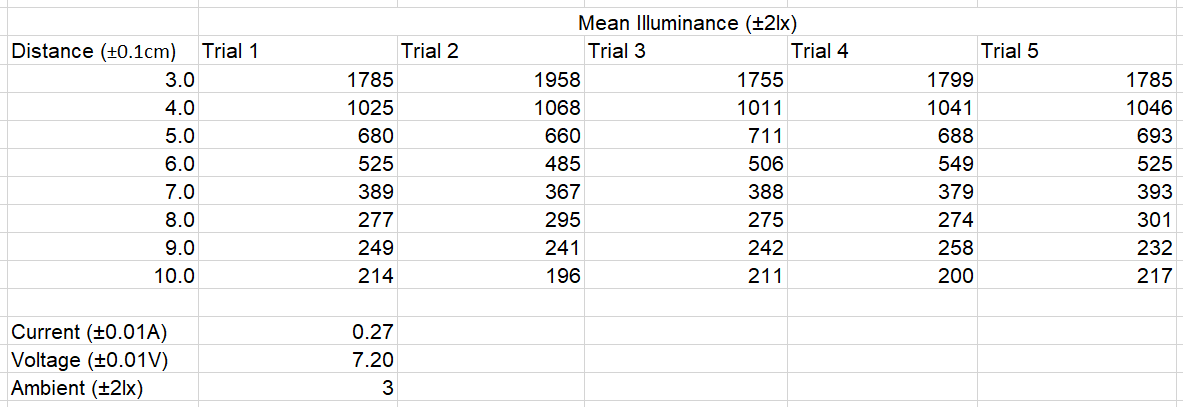
\includegraphics[width=\textwidth]{assets/rawdata.png}
    \caption{Unprocessed experimental data}
    \label{fig:raw}
\end{figure}

\subsection{Processing}
\paragraph{Notation}

Uncertainty: unc \quad Absolute uncertainty: $\Delta$unc \quad Relative uncertainty: \%unc


\subsubsection{Processing Power}
Power is defined in figure \ref{eq:work}:
\begin{align*}
\text{Power} &= \text{Current} \times \text{Voltage}\\
        &= 0.27\si{A} \times 7.20\si{V} \approx 1.94 \si{W}
\end{align*}

\textit{Uncertainty}: $\relun$W =  $\relun$A +  $\relun$V
\begin{align*}
    \relun \si{A} &= \frac{0.01}{0.27},\quad \relun \si{V} = \frac{0.01}{7.20}\\
    \relun \si{W} &\approx 0.038,\quad \absun \si{W} \approx 0.07\si{W}
\end{align*}

Therefore: $P = 1.94 \pm 0.07 \si{W}$

\subsubsection{Processing Illuminance}

\paragraphnl{Correcting for the ambient illuminance}
Subtract the each illuminance values by the ambient illuminance value (figure \ref{fig:corrected}).

\textit{Uncertainty}: $\absun$Corrected = $\absun$Measured + $\absun$Ambient
\begin{align*}
     \absun \text{Corrected} = 0.2 + 0.2 = 0.4\si{lx}
\end{align*}

\begin{figure}[H]
    \centering
    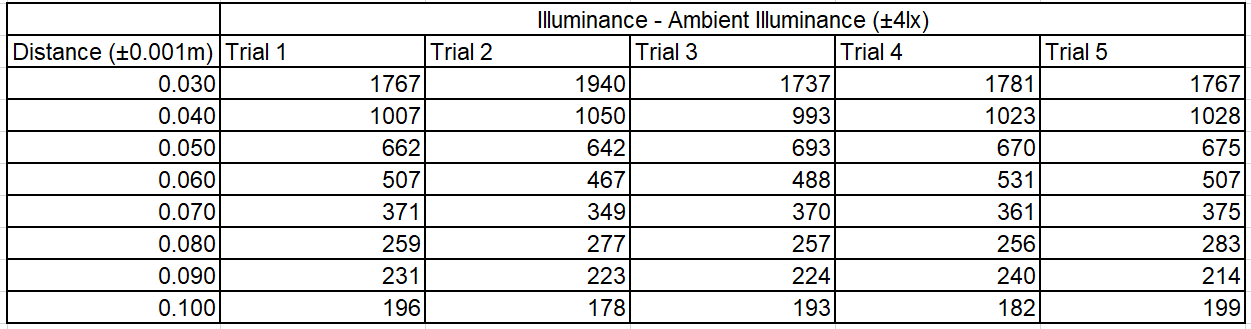
\includegraphics[scale=0.5]{assets/correcteddata.png}
    \caption{Corrected illuminance values}
    \label{fig:corrected}
\end{figure}

\paragraphnl{Averaging trial illuminances}
Average the measured illuminance. Additionally, the distances are converted into standard SI units in meters (figure \ref{fig:average}, graph \ref{gph:average}).

\textit{Uncertainty:} $\absun \text{illum.}_{\text{avg}} = \frac{\text{max}(\text{illum}.) - \text{min}(\text{illum}.)}{2}$

for distance 3cm:
\begin{align*}
 \absun \text{illuminance}_{\text{avg}} &= \frac{1940-1737}{2}\\
 &\approx 102 \,\si{lx}
\end{align*}


\begin{figure}[H]
    \centering
    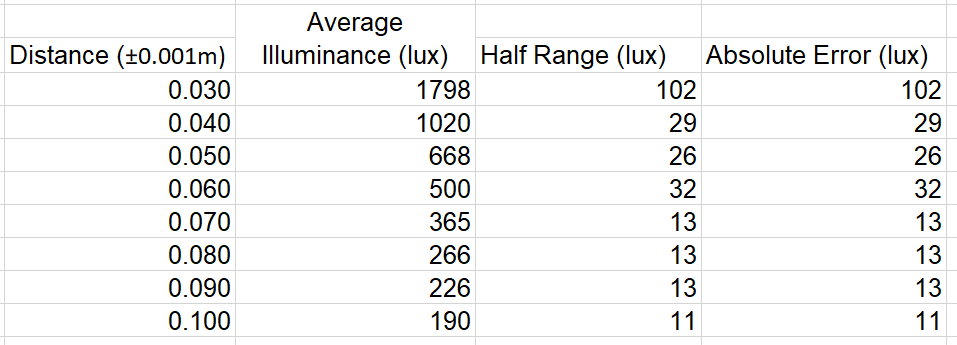
\includegraphics[scale=0.5]{assets/averagedata.png}
    \caption{Averaged illuminance values}
    \label{fig:average}
\end{figure}

\begin{figure}[H]
    \centering
    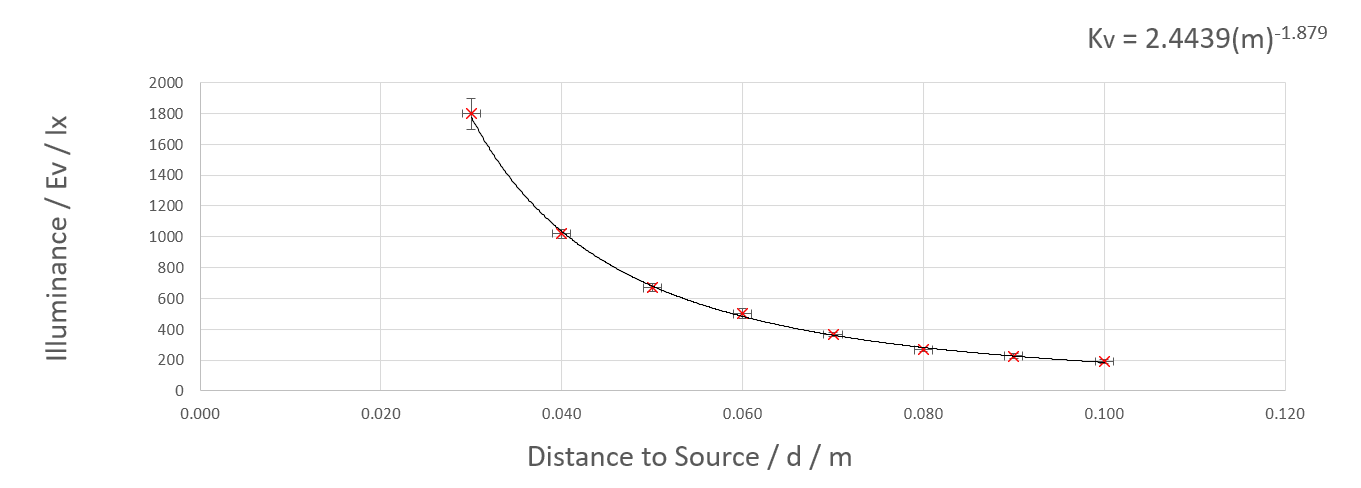
\includegraphics[width=\textwidth]{assets/averagegraph.png}
    \caption{Graph of the averaged illuminance values}
    \label{gph:average}
\end{figure}


\paragraphnl{Applying inverse squared transform on distance}
Graph \ref{gph:average} looks like an inverse squared graph, so I attempted to straighten it with $1/{\text{distance}}^2$ transformation. The transformation data and error is generated with Microsoft Excel (figure \ref{fig:tdata}, graph \ref{gph:tdata}).

\textit{Error bars}: $\relun 1/{\text{distance}}^2$ = $2 \times \relun \text{distance}$

\begin{figure}[H]
    \centering
    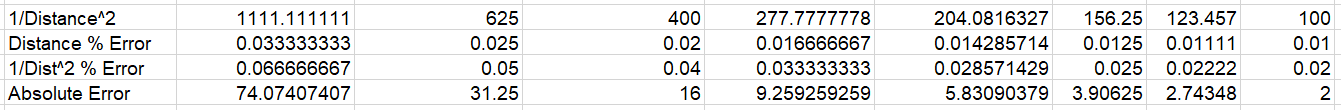
\includegraphics[width=\textwidth]{assets/transformdata.png}
    \caption{Transformed distance data}
    \label{fig:tdata}
\end{figure}

\begin{figure}[H]
    \centering
    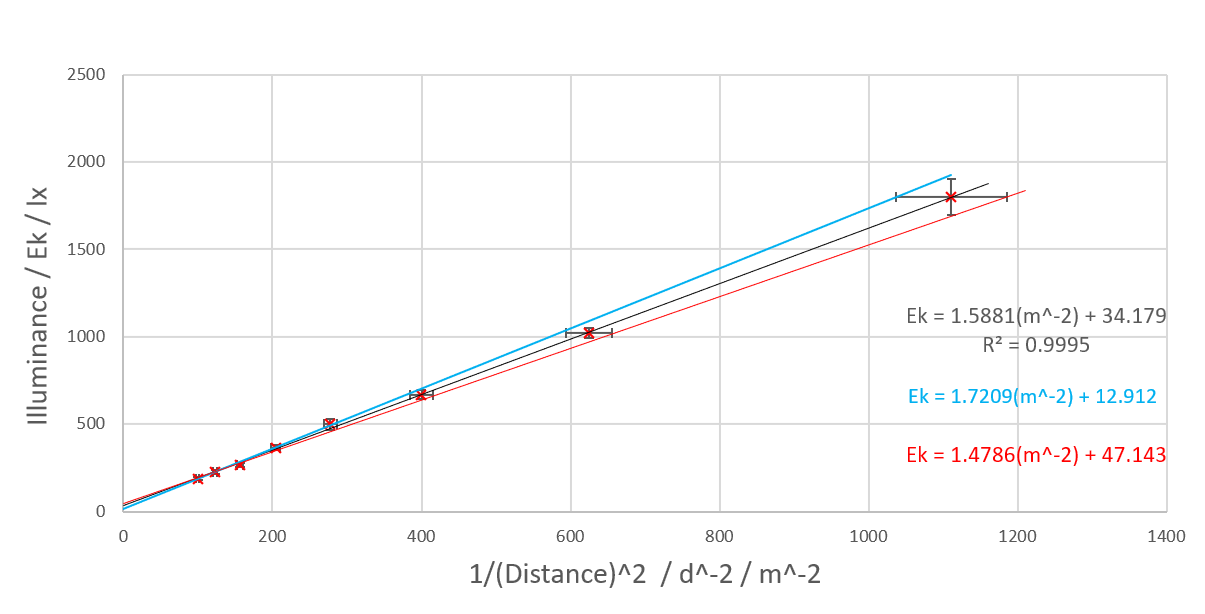
\includegraphics[width=\textwidth]{assets/transformgraph.png}
    \caption{Transformed distance graph}
    \label{gph:tdata}
\end{figure}

\paragraphnl{Gradient and Errors}
The justification for the horizontal error line of worst fits in figure \ref{gph:tdata} resides in the accuracy of the measuring devices: the percentage errors of the ruler are (for all values) larger than the percentage error of the light sensor, as indicated by the size of the error bars.


Higher gradient line of worst fit (HGLWF): 1.7209

Lower gradient line of worst fit (LGLWF): 1.4768

Gradient of line of best fit (GLBF): 1.5881

Half range: $\frac{1}{2} (\text{HGLWF} - \text{LGLWF})= \frac{1}{2}(1.7209-1.4768) \approx 0.121 \approx 12.1\% $

Final \% error: $12.1\%$

\textit{Uncertainty}: \% error x GLBF = 12.1\% of $1.59$ = 0.2 (1 sf)

Slope = $1.6 \pm 0.2$

Therefore, the relationship is summarized as in figure \ref{fig:rel}:
\begin{figure}[h!]
    \[
       E_v = (1.6 \pm 0.2) \frac{1}{s^2} + 49.2
    \]
    \caption{Experimental relationship between illuminance against distance from source}
    \label{fig:rel}
\end{figure}

\section{Conclusions}
\subsection{Result}

Following the data collection and some transformation for linearization, the relationship is summarized in figure \ref{fig:rel}. It seems that the data had supported my suspicion to a large extend. From graph \ref{gph:average}, one can see the that measured illuminance  greatly falls when the distance to source increases --- notice the distance scale. To create a linear curve, the illuminance ($E_v$) is plotted against the inverse square of the distance ($\frac{1}{s^2}$) shown in graph \ref{gph:tdata}. The small variance of the data points from the line of best fit is a strong evidence to support my hypothesis.

However, for the hypothesis also suggests that the relation curve should also intercept the y axis at point (0, 0), the lack of that feature in the graph suggests some systematical error are present --- the line of best fit has a positive intercept of $34.2 \si{lx}$ instead of $0 \si{lx}$. The existance of some systematic error shifting the curve upwards usually means a degree of inaccuracy, but judging from the small percentage of the error in respect to the values data points --- $34.2 / 1798 \approx 2\%$, the inaccuracy present here is tiny, further indicating a success in my method. Nevertheless, the systematic error could be caused by the erroneous reading of the ambient illuminance, parallax error in aligning the ruler, or by a lack of calibration of the light sensor.

Additionally, the experimental data contains a noticeable amount of uncertainties indicated by the large error bars, particularly at smaller distances. There also exists large random error in the illuminance measurement, as indicated by the high half ranges of the trials of illuminance measurements during averaging (figure \ref{fig:average}) --- sometimes to a degree of $102/1798 \approx 5.7\%$ at the distance of $3\si{cm}$. This is most likely caused by the fluctuation of the light level in the room, which is likely caused by the leakage of sunlight through the window blinds. This is also reflected in the gradient calculations, for the slope had a relatively large uncertainty of $12.1\%$, supporting the presence of large random errors. However, the averaging of the data seemed to reduce the effects of the error. The line of best fit passed through all 8 points of the independent variable, and had a very high R-squared value of $0.9995$ and R value of $\sqrt{0.9995} \approx 0.9997$. This shows a high level of correlation in the data. In conclusion, the raw dataset presented in figure \ref{fig:raw} is said to be highly accuracy but less precise, and contains medium amounts of uncertainty.

\subsection{Implications}

If we were to define the proportionality constant $\eta$ in figure \ref{eq:li} with parameter power, such that:

\begin{align*}
    \eta &= \frac{1}{4\pi A} \si{\ohm} K_{cd} \int_{0}^{\infty} V(\lambda) c(\lambda) \, d\lambda\\
    E_v &= \eta P \frac{1}{s^2},
\end{align*}

where $\eta$ is another constant, I can fulfill my motivation for this experiment. Notice the units of the constant $\eta$ is $(\frac{\si{lx}}{\si{W\per m^2}} = \frac{\si{lm}}{\si{W}})$, is a value that is only depended on the light source used. Therefore, the constant $\eta$ is a measure of the efficacy of the light-bulb used in the amount of luminous power produced per unit power. This is also known as the typical luminous efficacy, one that I can use to compare to other light-bulbs using an online database. Furthermore, the value can be used to compare efficiency of light-bulbs in your daily life, whether that is to save money, or like me, to appreciate how far lighting technology had advanced.

A division is needed to calculate the luminous efficacy $\eta$:
\begin{align*}
    \eta &= \frac{k}{P} = \frac{1.6 \pm 0.2}{1.94 \pm 0.07}\\
    &\approx 0.82 \pm 0.13 \si{lm\per W}.
\end{align*}

In comparison to the typical values shown in table \ref{tbl:leff}, the lab incandescent 5W light-bulb that I've used, which has a luminous efficacy value of $0.82 \pm 0.13 (\si{lm\per W})$, looks to be as efficient in producing light as a typical fireplace. This is unsurprising, as the outer glass casing of the bulb readily heats up when it is powered, indicating energy loss in the form of thermal energy. A suggestion is to made for the school physics department for a switch to safer (less temperature), and more energy efficient light-bulbs for general experiments.

\begin{table}[H]
    \centering
    \begin{tabular}{l|l}
        Category     & Luminous Efficacy (lm/W) \\ \hline
        Combustion   & 1-2                      \\
        Incandescent & 5-17.5                   \\
        Halogen      & 16.7-35                  \\
        Fluorescent  & 46-104.2                 \\
        LED          & 75-210
    \end{tabular}
    \caption{List of common luminous efficacy values of light sources \parencite{le_value1} \parencite{le_value2} \parencite{le_value3} \parencite{le_value4}}
    \label{tbl:leff}
\end{table}

\subsection{Reflection}

Here is a list on the handling of the controlled variables/potential error factors, and future improvements to be made.

\subsubsection{Random Errors}
\paragraph{Fluctuation of the outside light level} This is potentially a significant factor in creating a large uncertainty and low precision in the raw illuminance data. The advice would be to conduct the experiment at night, or in a totally blackout room without light pollution. This will increase the precision of the experiment and decrease the uncertainty on the luminous efficacy.

\paragraph{The sensitivity of the light sensor} Insignificant, for the equipment is properly taped down, removing the problem of a shaky hand.

\paragraph{The power supplied to the light-bulb}
Insignificant, for the power held stable during the experiment.

\subsubsection{Systematic Errors}
\paragraph{Environmental room intensity}
A potentially significant variable. The small but existent systematic error is likely to be caused by the erroneous measure of the ambient room light level. Performing the experiment in a blackout room or at night is likely to reduce the effects of the ambient room intensity and increase the accuracy of the dataset, possibility creating a curve that intercepts closer to 0 on the y axis.

\paragraph{The temperature of the bulb filament}
Insignificant, for the power is kept below the operating power limit and a lack of systematic decreasing illuminance during trials.

\paragraph{Parallax placements of the ruler}
A potentially significant variable. For the wooden ruler have depth, an angled top-down view to place the ruler is likely to result in parallax errors, thus systematically displacing the measured distances. It may be wise to have used a paper with beforehand markings of the distances, which is likely in reducing the systematic error shown in the curve, and potentially help bring the intercept closer to point (0,0).

\paragraph{Accuracy of the light sensor}
A variable that I was the most concerned about. This may be the largest cause of the systematic error. I could follow a lengthy calibration test listed on the manufacture's website against a factory calibrated source, which will decrease the systematic error and increase the accuracy of the data.

\nocite{*}
\printbibliography



\end{document}
